
% Default to the notebook output style

    


% Inherit from the specified cell style.


    
\documentclass[11pt]{article}

\usepackage{graphicx}

\author{Maximilian Mayerl, Alexander Schl\"ogl, Benedikt Wimmer}
\title{Assignment 1, Report}

\begin{document}


\maketitle

    

    
\section{Implementation}\label{implementation}

Implementing the different solvers was fairly straight-forward. The
different update procedures between the solvers are as follows:

\subsection{Forward Euler}\label{forward-euler}

\begin{enumerate}
\item
  Calculate forces for \emph{t}
\item
  Calculate acceleration for \emph{t}
\item
  Calculate position for \emph{t+h}
\item
  Calculate velocity for \emph{t+h}
\end{enumerate}

\subsection{Symplectic Euler}\label{symplectic-euler}

The only difference between the forward and symplectic Euler is the
order of the calculations. 1. Calculate position for \emph{t+h} 2.
Calculate forces for \emph{t} (using \emph{x(t+h)}) 3. Calculate
acceleration for \emph{t} 4. Calculate position for \emph{t+h}

\textbf{Note:} we used the variant of the symplectic Euler which uses
the new position, not the new velocity.

\subsection{Leapfrog}\label{leapfrog}

The leapfrog solver works in two steps: 1. Update the velocity at
\emph{t-h/2} 2. Update the position at \emph{t}

This provides better accuracy (\emph{\textbf{O}(h3)}). For calculating
the damping force, the velocity for \emph{t} is approximated. It is
unclear how this affects the accuracy.

\textbf{Note:} because we cannot perform calculations in half-steps in
our framework, we halved the step size and updated the positions and
velocities every other update respectively. This means that instead of
using \emph{dt} we use \emph{2 dt} for full update steps, and \emph{dt}
for the initialization step.

\subsection{Midpoint}\label{midpoint}

The midpoint solver works as follows: 1. Calculate positions and
velocities for \emph{t+h/2} 2. Calculate forces for \emph{t+h/2} using
the new positions and veloicities 3. Calculate the positions for
\emph{t+h} based off of the position for \emph{t} and the velocity for
\emph{t+h/2} 4. Calculate the velocities for \emph{t+h} similarly

\subsection{Changes to the code}\label{changes-to-the-code}

Most of the changes we implemented were in the \textbf{Exercise.cpp}.
However, based on OOP considerations, we decided to implement the
application of force in the \textbf{Spring.cpp}, to save us the check if
a point is contained in a spring. This does not affect solver behaviour,
as the calculation of spring forces is fixed for all methods.

In addition, we also added internal damping for the springs, based on
the internal friction that occurs when deforming the spring. Spring
damping is calculated based on a spring damping coefficient and the
relative velocity of the connected mass-points. Only relative velocity
parallel to the direction of the spring is taken into account for this
damping. The default spring damping coefficient is \emph{0}.

\section{Stability}\label{stability}

This section provides an analysis of the stability for the different
solvers and different test cases. We describe a system as stable if it
comes to rest at some point and the total energy shrinks. An unstable
system results in an "explosion", where all non-fixed mass points shoot
out of view. We could not observe any difference regarding the testcase.
A(n) (un)stable system was (un)stable for all 3 testcases(spring,
hanging, falling). In general the stepsize and spring stiffness had the
biggest impact on stability. Since there are infinitely many possible
scenarios we decided to start with the default values and from there
alter stepsize and spring stiffness seperately up to a change in
stability. Default stepsize: 0.003, stiffness: 60

\begin{enumerate}
\item
  \textbf{Forward Euler}: Unstable for the default parameters. Stable
  for stepsize \textless{}= 0.001 or stiffness \textless{}= 20
\item
  \textbf{Symplectic Euler}: Stable for the default parameters. Unstable
  for stepsize \textgreater{}= 0.1 or stiffness \textgreater{}= 69000
\item
  \textbf{Leapfrog}: Stable for the default parameters. Unstable for
  stepsize \textgreater{}= 0.1 or stiffness \textgreater{}= 69000
\item
  \textbf{Midpoint}: Stable for the default parameters. Unstable for
  stepsize \textgreater{}= 0.04 or stiffness \textgreater{}=2500
\end{enumerate}

\textbf{Result}: The forward Euler solver is by far the least stable.
The Symplectic Euler and Leapfrog solvers are very robust and very
similar in their stability behaviour. The Midpoint solver, while being
the most accurate is not as stable as the Symplectic Euler or the
Leapfrog. It is very susceptible instabilities at larger step sizes.

\section{Comparison to exact
solution}\label{comparison-to-exact-solution}

The first plot in the following figure shows the behaviour of the
different solvers, as well as the analytical solution. The analytical
solution was obtained using the start values \emph{x(0) = 0} and
\emph{x'(0) = 0}.

As visible, the most divergence from the analytical solution is in
frequency. The solvers that comes closest, however, are the leapfrog and
midpoint solvers. These are also the solvers with the highest order of
accuracy. Interesting to note is the fact that the approximation of
velocity for the calculation of acceleration in the leapfrog solver does
not cause greater error, as this is the solver that most accurately
approximates the decay of amplitude in the oscillation.

The second plot shows the absolute error of the different solver methods
compared to the analytical solution. Improtant to note here is the fact
that the error stems from a difference in frequency, not amplitude. Thus
the error is better observed in the plot of amplitudes.
\begin{figure}[h]
    \centering
    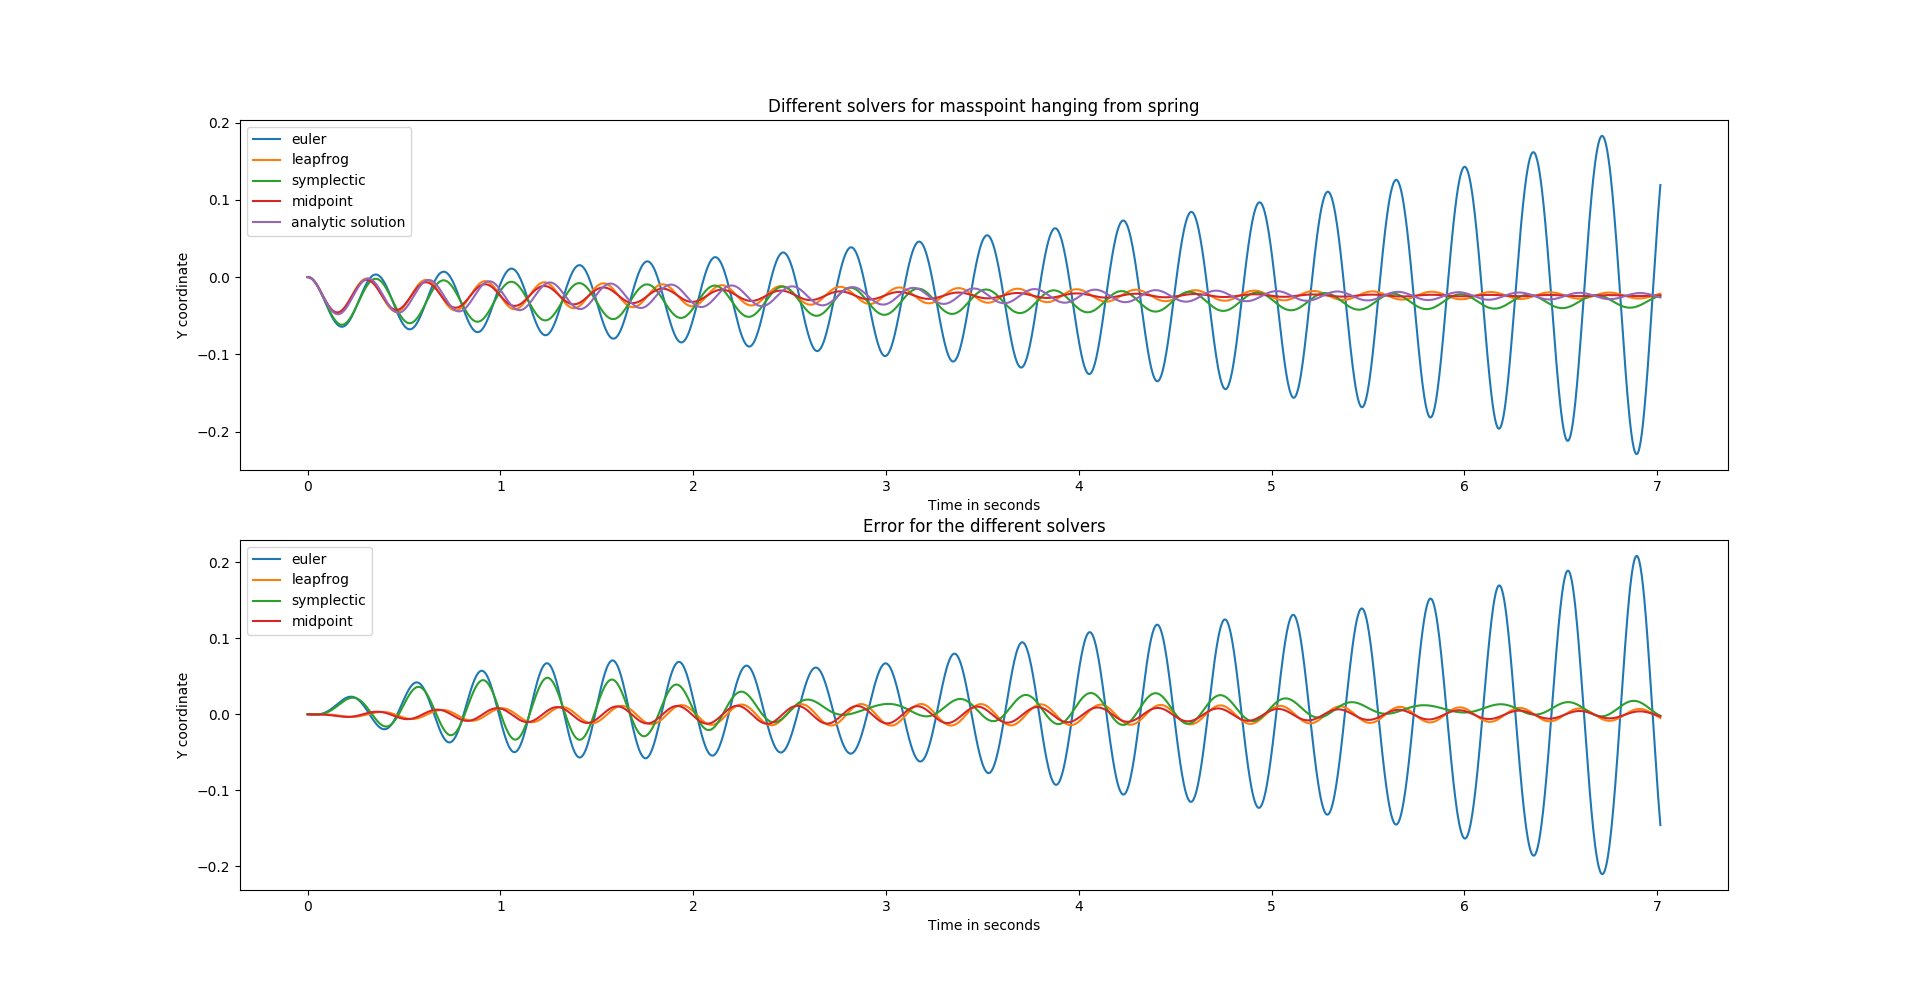
\includegraphics[width=\textwidth]{plots.png}
\end{figure}
    

    % Add a bibliography block to the postdoc
    
    
    
    \end{document}
